\documentclass[border={20pt 20pt 20pt 20pt},preview]{standalone}

\usepackage{amssymb}
\usepackage{amsmath}
\usepackage{subcaption}

\usepackage{pgfplots}
\usepackage{pgfplotstable}
\pgfplotsset{compat=1.16}

\usepackage{xcolor}

\usepackage{tikz}
\usetikzlibrary{patterns}
\usetikzlibrary{positioning}
\usetikzlibrary{decorations.pathmorphing}

\begin{document}

\begin{figure}[ht!]
\centering
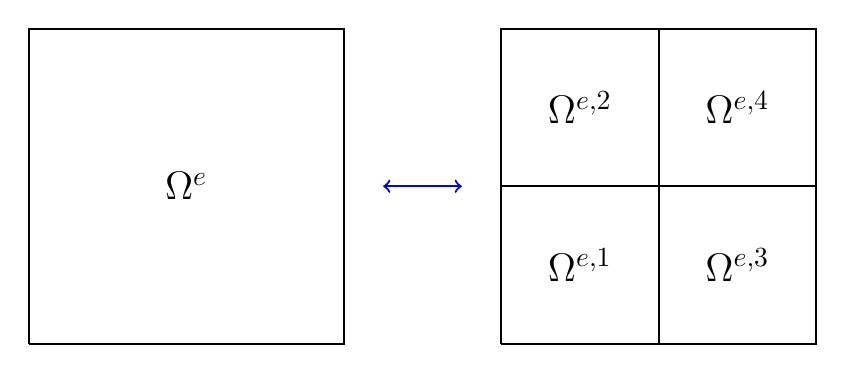
\begin{tikzpicture}

\coordinate(A) at (0, 0);
\coordinate(B) at (4, 0);
\coordinate(C) at (4, 4);
\coordinate(D) at (0, 4);

\coordinate(E) at (6, 0);
\coordinate(F) at (10, 0);
\coordinate(G) at (10, 4);
\coordinate(H) at (6, 4);

\coordinate(I) at (8, 0);
\coordinate(J) at (8, 4);
\coordinate(K) at (6, 2);
\coordinate(L) at (10, 2);

\draw [black, thick] (A) -- (B) -- (C) -- (D) -- (A);
\node[] (a) at (2,2) {\Large $\Omega^e$};

\coordinate(M) at (4.5, 2);
\coordinate(N) at (5.5, 2);

\draw [blue, thick, <->] (M) -- (N);

\draw [black, thick] (E) -- (F) -- (G) -- (H) -- (E);
\draw [black, thick] (I) -- (J);
\draw [black, thick] (K) -- (L);

\node[] (a) at (7,1) {\Large $\Omega^{e,1}$};
\node[] (a) at (7,3) {\Large $\Omega^{e,2}$};
\node[] (a) at (9,1) {\Large $\Omega^{e,3}$};
\node[] (a) at (9,3) {\Large $\Omega^{e,4}$};

\end{tikzpicture}
\caption*{Example of refinement (right arrow) and
coarsening (left arrow) in two dimensions.}
\end{figure}

\end{document}
